Industrial robots, and in particular manipulating robots, 
have a wide range of applications in a variety of sectors and 
offer many advantages, including increased productivity, accuracy 
and safety. Certain types of robots may be better suited to a particular 
application than others.
\begin{itemize}[itemsep=0pt]
    \item Welding
    \item Material Handling
    \item Assembly
    \item Painting and Coating
    \item Packaging
    \item Inspection and Quality Control
    \item Machine Tending
    \item Surgery and Medical Procedures
    \item Research and Development
    \item Education and Training
    \item Cleaning and Maintenance
\end{itemize}

\begin{figure}[H]
	\centering
	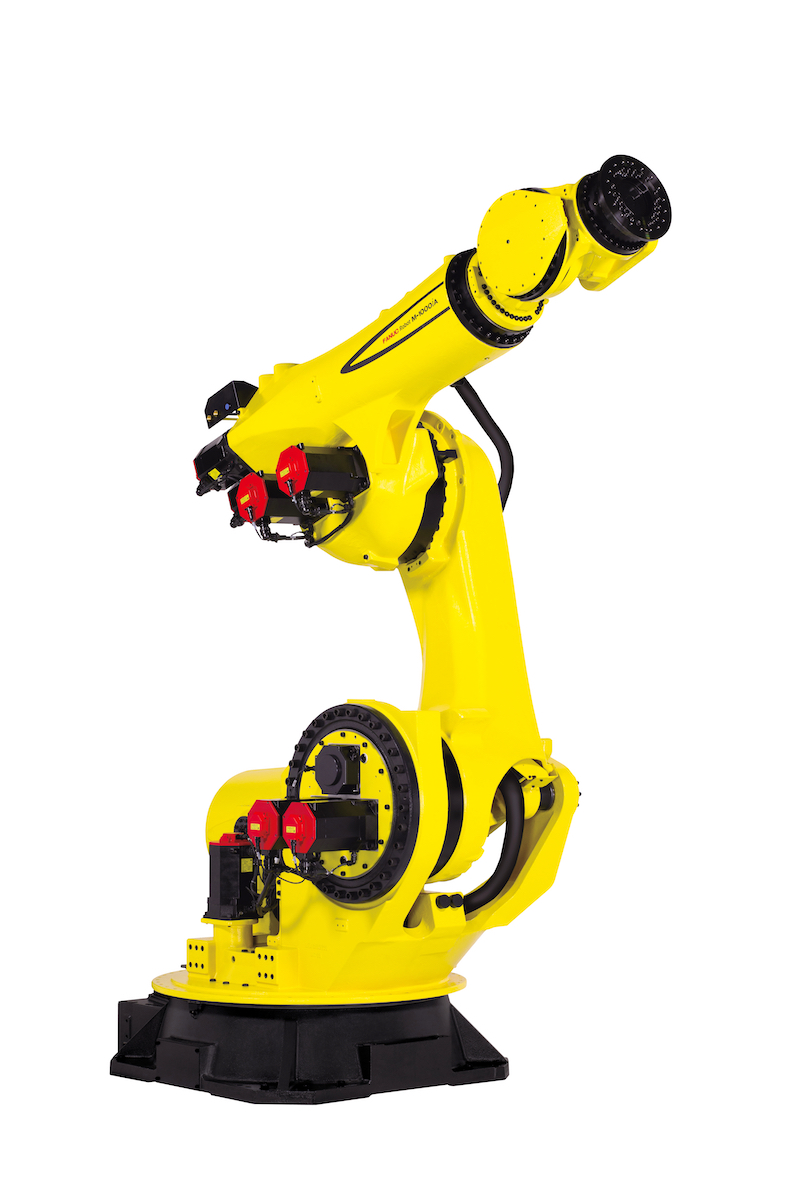
\includegraphics[width=0.3\textwidth]{Src/images/Robot.jpg}
	\caption{Indusrial robot arm}
\end{figure}

One of the main characteristics of any robot arm is the number of degrees of freedom(DoF), which is characterised by the set of motion axis parameters that the robot has.  It describes the freedom of movement of the robot arm or manipulator in its workspace.  The degrees of freedom of a robot arm are determined by the number of joints it has, each of which provides a specific axis of motion.

The degrees of freedom of the robot arm can be classified in one of two possible ways:
\begin{itemize}
    \item Linear Motion (Translational DoF)
    \item Rotational Motion (Rotational DoF)
\end{itemize}

Manipulator robots can be classified on the basis of their structure and movement capabilities. Each type is suitable for each application, rotating joints and often the preferred choice for tasks that involve reaching, grasping and positioning objects, as they allow for more flexible movement in a variety of directions. In scenarios where precise linear motion is required, such as assembly lines where components need to be moved in a straight line, prismatic couplings can be used. But it is not uncommon to use two types of motion in a robot design and they have become widespread.

There is no strict dependency on which type of robot arm should be used in a particular case. The choice of robot arm will still get the job done, but the right robot is necessary to maximise productivity and cost savings.

